\documentclass{report}
\usepackage[spanish]{babel}
\newtheorem{lemma}{Lema}

\renewcommand{\theenumii}{\roman{enumii}}
\usepackage[spanish]{babel}
\usepackage[utf8x]{inputenc}
\usepackage{amsmath}
\usepackage{graphicx}
\usepackage[colorinlistoftodos]{todonotes}
\usepackage{enumitem}
\usepackage{listings}
\usepackage{verbatim}
\usepackage{eurosym}
\usepackage[export]{adjustbox}
\usepackage{amssymb}
\usepackage{bussproofs}
\usepackage{amsmath}
\usepackage{tikz}
\usepackage{xcolor}
\usepackage{listings}
\usepackage{titletoc}
\usepackage{hyperref}

\hypersetup{
  colorlinks=true,
  linkcolor=black,
  urlcolor=blue,
  citecolor=black
}

\newcommand{\coverPage}[6]{%
%----------------------------------------------------------------------------------------
%	COVER START
%----------------------------------------------------------------------------------------
\begin{titlepage}

    \newcommand{\HRule}{\rule{\linewidth}{0.5mm}}
    \newcommand{\department}{#1}
    \newcommand{\course}{#2}
    \newcommand{\titleValue}{#3}
    \newcommand{\subtitleValue}{#4}
    \newcommand{\authorName}{#5}

    \center

    %----------------------------------------------------------------------------------------
    %	HEADER
    %----------------------------------------------------------------------------------------
    
\includegraphics{images/logo_usa.png}
    \vspace{0.5cm}
    \textsc{\Large \department}\\[0.5cm]
    \textsc{\Large \course}\\[0.5cm]
    \vfill

    %----------------------------------------------------------------------------------------
    %	TITLE
    %----------------------------------------------------------------------------------------

    \HRule\\
    \Huge
    \textbf{\titleValue}\\[0.5cm]
    \Large
    \textbf{\subtitleValue}\\
    \HRule\\[0.5cm]

    %----------------------------------------------------------------------------------------
    %	AUTHOR AND DATE
    %----------------------------------------------------------------------------------------

    \vfill
    \Large
    \textit{\authorName}\\
    {\large \today}\\[2cm]

\end{titlepage}
%----------------------------------------------------------------------------------------
%	COVER END
%----------------------------------------------------------------------------------------
}

\begin{document}
    \coverPage{ Matemáticas }{ Cálculo Integral y Series }{ Taller 1 }{  }{ Alexander Mendoza }{\today}

    \section*{Spivak Capítulo 13}

    \begin{enumerate}
        \item Demostrar que $\int_{0}^{b}x^3dx = \dfrac{b^4}{4}$.

        Consideremos la partición de [0, b] $P_n$ tal que $t_i - t_{i-1} = \dfrac{b}{n}$, así $t_0 = 0, t_1 = \dfrac{b}{n}, \dots , t_i =\dfrac{ib}{n}$. Con esto, sabemos que
        $$m_i = t_{i-1}^3 = \left((i-1)\dfrac{b}{n}\right)^3$$
        $$M_i = t_{i}^3 = \left(i\dfrac{b}{n}\right)^3$$

        Luego

        \begin{align*}
            L(f, P_n) &= \sum_{i=1}^{n}\left((i-1)\dfrac{b}{n}\right)^3\dfrac{b}{n}\\
            &= \sum_{i=1}^{n}(i-1)^3\dfrac{b^4}{n^4}\\
            &= \dfrac{b^4}{n^4} \sum_{i=1}^{n}(i-1)^3\\
            &= \dfrac{b^4}{n^4} \sum_{i=1}^{n-1}i^3\\
            &= \dfrac{b^4}{n^4} \left[\dfrac{n(n-1)}{2}\right]^2\\
            &= \dfrac{b^4}{4} \dfrac{(n-1)^2}{n^2}
        \end{align*}

        Con esto podemos observar que cuando $n$ se hace tan grande cuanto se quiera, $L(f, P_n)$ tiende a $\dfrac{b^4}{4}$. Continuamos de manera similar para $U(f, P_n)$

        \begin{align*}
            U(f, P_n) &= \sum_{i=1}^{n}\left(i\dfrac{b}{n}\right)^3\dfrac{b}{n}\\
            &= \sum_{i=1}^{n}i^3\dfrac{b^4}{n^4}\\
            &= \dfrac{b^4}{n^4} \sum_{i=1}^{n}i^3\\
            &= \dfrac{b^4}{n^4} \left[\dfrac{n(n+1)}{2}\right]^2\\
            &= \dfrac{b^4}{4} \dfrac{(n+1)^2}{n^2}
        \end{align*}

        Ahora calculemos la diferencia de las sumas

        \begin{align*}
            U(f, P_n) - L(f, P_n) &= \dfrac{b^4}{4} \dfrac{(n+1)^2}{n^2} - \dfrac{b^4}{4} \dfrac{(n-1)^2}{n^2}\\
            &= \dfrac{b^4}{4} \left[\dfrac{(n+1)^2}{n^2} - \dfrac{(n-1)^2}{n^2}\right]\\
            &= \dfrac{b^4}{4} \left(\dfrac{n^2+2}{n^2}\right)\\
            &= \dfrac{b^4}{n}
        \end{align*}

        De esta manera, dado $\epsilon > 0$ si $n > \dfrac{b^4}{\epsilon}$, entonces

        $$U(f, P_n) - L(f, P_n) = \dfrac{b^4}{n} < \epsilon$$

        Así, dado cualquier $\epsilon > 0$, podemos encontrar una partición $P_n$ de $[0,b]$ tal que $U(f, P_n) - L(f, P_n) < \epsilon$. Por lo tanto, $f$ es integrable. Luego como tanto $U(f, P_n)$ y $L(f, P_n)$ se aproximan a $\frac{b^4}{4}$ dado un $n$ lo suficiente mente grande, $\frac{b^4}{4}$ es el único número tal que

        $$L(f, P_n) = \dfrac{b^4}{4} \dfrac{(n-1)^2}{n^2} \leq \dfrac{b^4}{4} \leq \dfrac{b^4}{4} \dfrac{(n+1)^2}{n^2} = U(f, P_n)$$

        Por lo tanto $\int_{0}^{b} x^3 dx = \dfrac{b^4}{4}$.

        \item Demostrar que $\int_{0}^{b}x^4dx = \dfrac{b^5}{5}$.

        Consideremos la partición de [0, b] $P_n$ tal que $t_i - t_{i-1} = \dfrac{b}{n}$, así $t_0 = 0, t_1 = \dfrac{b}{n}, \dots , t_i =\dfrac{ib}{n}$. Con esto, sabemos que
        $$m_i = t_{i-1}^4 = \left((i-1)\dfrac{b}{n}\right)^4$$
        $$M_i = t_{i}^4 = \left(i\dfrac{b}{n}\right)^4$$

        Luego

        \begin{align*}
            L(f, P_n) &= \sum_{i=1}^{n}\left((i-1)\dfrac{b}{n}\right)^4\dfrac{b}{n}\\
            &= \sum_{i=1}^{n}(i-1)^4\dfrac{b^5}{n^5}\\
            &= \dfrac{b^5}{n^5} \sum_{i=1}^{n}(i-1)^4\\
            &= \dfrac{b^5}{n^5} \sum_{i=1}^{n-1}i^4\\
            &= \dfrac{b^5}{n^5} \dfrac{n(n-1)(2n-1)(3n^2-3n-1)}{30}\\
            &= \dfrac{b^5}{30} \dfrac{n(n-1)(2n-1)(3n^2-3n-1)}{n^5}\\
            &= \dfrac{b^5}{30} \left[6 + \dfrac{5(2-3n)n^2-1}{n^4}\right]\\
            &= \dfrac{b^5}{5} + \dfrac{b^5 5(2-3n)n^2-1}{30n^4}
        \end{align*}

        Con esto podemos observar que cuando $n$ se hace tan grande cuanto se quiera, $L(f, P_n)$ tiende a $\dfrac{b^4}{4}$. Continuamos de manera similar para $U(f, P_n)$

        \begin{align*}
            U(f, P_n) &= \sum_{i=1}^{n}\left(i\dfrac{b}{n}\right)^4\dfrac{b}{n}\\
            &= \sum_{i=1}^{n}i^4\dfrac{b^5}{n^5}\\
            &= \dfrac{b^5}{n^5} \sum_{i=1}^{n}i^4\\
            &= \dfrac{b^5}{n^5} \dfrac{n(n+1)(2n+1)(3n^2+3n-1)}{30}\\
            &= \dfrac{b^5}{30} \dfrac{n(n+1)(2n+1)(3n^2+3n-1)}{n^5}\\
            &= \dfrac{b^5}{30} \left[6 + \dfrac{5(2+3n)n^2-1}{n^4}\right]\\
            &= \dfrac{b^5}{5} + \dfrac{b^5 5(2+3n)n^2-1}{30n^4}
        \end{align*}

        Ahora calculemos la diferencia de las sumas

        \begin{align*}
            U(f, P_n) - L(f, P_n) &= \dfrac{b^5}{5} + \dfrac{b^5 5(2+3n)n^2-1}{30n^4} - \dfrac{b^5}{5} + \dfrac{b^5 5(2-3n)n^2-1}{30n^4}\\
            &= \frac{b^5}{n}
        \end{align*}

        De esta manera, dado $\epsilon > 0$ si $n > \dfrac{b^4}{\epsilon}$, entonces

        $$U(f, P_n) - L(f, P_n) = \dfrac{b^5}{n} < \epsilon$$

        Así, dado cualquier $\epsilon > 0$, podemos encontrar una partición $P_n$ de $[0,b]$ tal que $U(f, P_n) - L(f, P_n) < \epsilon$. Por lo tanto, $f$ es integrable. Luego como tanto $U(f, P_n)$ y $L(f, P_n)$ se aproximan a $\frac{b^5}{5}$ dado un $n$ lo suficiente mente grande, $\frac{b^5}{5}$ es el único número tal que

        $$L(f, P_n) = \dfrac{b^5}{5} + \dfrac{b^5 5(2-3n)n^2-1}{30n^4} \leq \dfrac{b^5}{5} \leq \dfrac{b^5}{5} + \dfrac{b^5 5(2+3n)n^2-1}{30n^4} = U(f, P_n)$$

        Por lo tanto $\int_{0}^{b} x^3 dx = \dfrac{b^5}{5}$.

        \setcounter{enumi}{4}
        \item Obtener sin cálculos
            \begin{enumerate}
                \item $\int_{-1}^{1}x^3\sqrt{1-x^2}dx$

                La gráfica de la función es la siguiente:

                \begin{center}
                    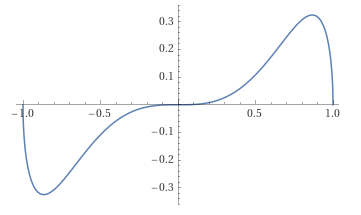
\includegraphics[width=.5\textwidth]{images/grafica1.png}
                \end{center}

                Observando la función, podemos observar que es impar, esto se puede verificar ya que

                $$ - (x^3\sqrt{1-x^2}) = (-x)^3\sqrt{1-(-x)^2}$$

                Luego $\int_{-1}^{1}x^3\sqrt{1-x^2}dx = 0$, esto se puede observar gráficamente ya que el área debajo del eje $x$ es igual al área sobre el eje, por lo cual se cancelan.

                \item $\int_{-1}^{1}(x^5+3)\sqrt{1-x} dx$

                Primero manipulemos la expresión para que sea más fácil de trabajar,

                $$\int_{-1}^{1}(x^5+3)\sqrt{1-x}dx = \int_{-1}^{1}x^5\sqrt{1-x}dx + \int_{-1}^{1}3\sqrt{1-xdx}$$

                Observemos que $x^5\sqrt{1-x}$ es impar, por lo tanto $\int_{-1}^{1}x^5\sqrt{1-x} = 0$. Además observemos que $\sqrt{1-xdx}$ es una función par, por lo tanto  $\int_{-1}^{1}\sqrt{1-xdx} = 2\int_{0}^{1}\sqrt{1-xdx}$. Por último observemos que $\sqrt{1-x}$ es la función del círculo unitario, por lo tanto $\int_{0}^{1}\sqrt{1-xdx} = \pi/4$  así tenemos los siguiente

                \begin{align*}
                    \int_{-1}^{1}(x^5+3)\sqrt{1-x}dx &= \int_{-1}^{1}x^5\sqrt{1-x}dx + \int_{-1}^{1}3\sqrt{1-xdx}\\
                    &= 0 + 3\int_{-1}^{1}\sqrt{1-xdx}\\
                    &= 6\int_{0}^{1}\sqrt{1-xdx}\\
                    &= 6 \left(\dfrac{\pi}{4}\right)\\
                    &= \frac{3\pi}{4}
                \end{align*}
            \end{enumerate}
            \setcounter{enumi}{6}
            \item Decidir cuáles de las siguientes funciones siguientes son integrables sobre $[0,2]$, y calcular la integral cuando sea posible.
            \begin{enumerate}
                \item $f(x) = \begin{cases}
                    x, & 0\leq x < 1\\
                    x-2, & 1\leq x \leq 2
                \end{cases}$

                La función es integrable y su integral se calcula de la siguiente manera

                \begin{align*}
                    \int_{0}^{2}f(x)dx &= \int_{0}^{1}xdx + \int_{1}^{2}x-2dx\\
                    &= \int_{0}^{1}xdx + \int_{1}^{2}x -\int_{1}^{2}2dx\\
                    &= \left(\dfrac{1^2}{2} - \dfrac{0^2}{2}\right) + \left(\dfrac{2^2}{2} - \dfrac{1^2}{2}-2(2-1)\right)\\
                    &= \dfrac{1}{2} + 2 - \dfrac{1}{2} - 4 + 2\\
                    &= 0
                \end{align*}

                \item $f(x) = x + [x]$

                La función es integrable y su integral se calcula de la siguiente manera

                \begin{align*}
                    \int_{0}^{2}x+[x]dx &= \int_{0}^{2} xdx + \int_{0}^{2}[x]dx\\
                    &= \int_{0}^{2} xdx + \int_{0}^{1}[x]dx + \int_{1}^{2} [x] dx\\
                    &= \left(\dfrac{2^2}{2} - \dfrac{0^2}{2}\right) + 0(1-0) + 1(2-1)\\
                    &= 3
                \end{align*}

                \item $f(x) = \begin{cases}
                    \dfrac{1}{\left[\frac{1}{x}\right]}, & 0 < x \leq 1\\
                    0, & x=0 \text{ o } x > 1
                \end{cases}$

                La gráfica de la función es la siguiente\\
                \begin{center}
                    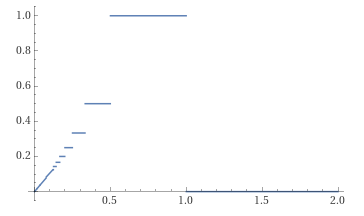
\includegraphics[width=.5\textwidth]{images/grafica2.png}
                \end{center}
            \end{enumerate}
    \end{enumerate}
\end{document}
